\documentclass[11pt, leqno]{beamer}
%\usetheme{Montpellier}
\usetheme{Dresden}
\usepackage[utf8]{inputenc}
\usepackage[english]{babel}
\usepackage{amsmath}
\usepackage{amsfonts}
\usepackage{amssymb}
\usepackage{graphicx}
\usepackage[compatibility=false]{caption}
\usepackage{subcaption}
\usepackage{multicol}

\usepackage{siunitx}
\usepackage{wrapfig}
%\usepackage{float}

\usepackage{caption}
\usepackage{subcaption}

\author{Davide Bazzanella}
\title{Thermal tuning of phase-matching in a multimodal SOI waveguide with $\chi^{(3)}$ non linearity}
\date{28 settembre 2015} 
%\textsc{\LARGE \textbf{DEPARTMENT OF PHYSICS}}\\[0.5cm]
%\textsc{\LARGE \textbf{DEGREE IN PHYSICS – LAUREA IN FISICA}}\\[2.5cm]
%\textsc{\Large THESIS}\\[1.3cm]



%\setbeamercovered{transparent} 
\setbeamertemplate{navigation symbols}{} 
%\logo{} 
%\institute{} 
%\subject{} 

\usepackage{lmodern}
\newcommand{\frameofframes}{/}
\newcommand{\setframeofframes}[1]{\renewcommand{\frameofframes}{#1}}

\setframeofframes{of}
\makeatletter
\setbeamertemplate{footline}
  {%
    \begin{beamercolorbox}[colsep=1.5pt]{upper separation line foot}
    \end{beamercolorbox}
    \begin{beamercolorbox}[ht=2.5ex,dp=1.125ex,%
      leftskip=.3cm,rightskip=.3cm plus1fil]{author in head/foot}%
      \leavevmode{\usebeamerfont{author in head/foot}\insertshortauthor}%
      \hfill%
      {\usebeamerfont{institute in head/foot}\usebeamercolor[fg]{institute in head/foot}\insertshortinstitute}%
    \end{beamercolorbox}%
    \begin{beamercolorbox}[ht=2.5ex,dp=1.125ex,%
      leftskip=.3cm,rightskip=.3cm plus1fil]{title in head/foot}%
      {\usebeamerfont{title in head/foot}\insertshorttitle}%
      \hfill%
      {\usebeamerfont{frame number}\usebeamercolor[fg]{frame number}\insertframenumber~\frameofframes~\inserttotalframenumber}
    \end{beamercolorbox}%
    \begin{beamercolorbox}[colsep=1.5pt]{lower separation line foot}
    \end{beamercolorbox}
  }
\makeatother

\begin{document}

\begin{frame}
\titlepage
\end{frame}

\begin{frame}{Outline}
%\footnotesize
\tableofcontents
\end{frame}

\section{Introduction}
\begin{frame}{Introduction}
	
	\textbf{Research field}:\\
	bio-sensors, gas sensors and bio-medical instrumentation
	
	\vspace{5pt}
	\textbf{Problem}:\\
	lack of sources/sensors in the MIR (3-10\si{\um})
	
	\begin{figure}
		\centering
		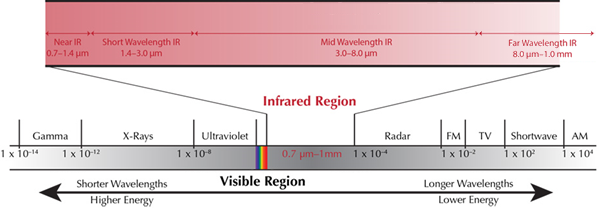
\includegraphics[width=\textwidth]{spectrum2.png}
	\end{figure}
\end{frame}
\begin{frame}
	\textbf{Solution}:\\
	frequency down convertion from NIR/VIS sources to MIR\\
	frequency up convertion from MIR signals to NIR/VIS sensor

	\begin{figure}[hb]
%		\centering
%		\begin{subfigure}[c]{.725\textwidth}
			\centering
			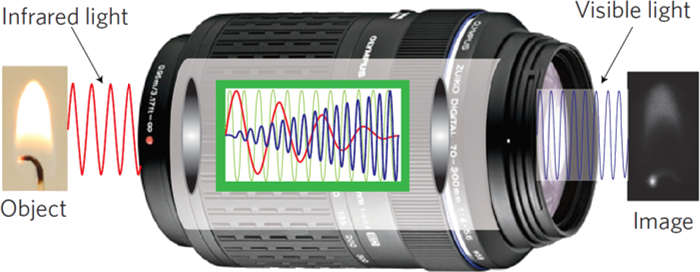
\includegraphics[width=.75\textwidth]{upconversion2_short.png}
%			\caption{}
%		\end{subfigure}
%		\hspace{0.02\textwidth}
%		\begin{subfigure}[c]{.225\textwidth}
%			\centering
%			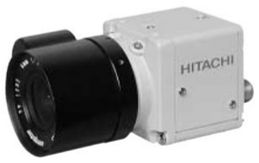
\includegraphics[width=\textwidth]{upconverter_HITACHI.png}
%			\caption{}
%		\end{subfigure}
	\end{figure}	
%	\vspace{15pt}
	\textbf{Aim}:\\
	Develop integrated frequency converter tunable with temperature
\end{frame}

\section{Nonlinear Optics}
\begin{frame}{Nonlinear Optics}
	Frequency convertion employs nonlinear properties of materials
	\begin{equation}
		\textbf{P} = \varepsilon_0 \left( \chi^{(1)} \cdot \textbf{E} + \chi^{(2)} : \textbf{E}^2 + \chi^{(3)} \vdots \textbf{E}^3 + \cdots \right) = \mathrm{\textbf{P}_L} + \mathrm{\textbf{P}_{NL}}
		\label{eq_P_general}
	\end{equation}
	\begin{wrapfigure}{r}{0.33\textwidth}
		\centering
		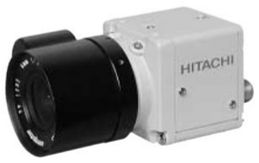
\includegraphics[width=.3\textwidth]{upconverter_HITACHI.png}
	\end{wrapfigure}
	\begin{itemize}
	\item	$\chi^{(1)}$	:	linear part
	\item	$\chi^{(2)}$	:	2$^{nd}$ order nonlinearity\\ \hspace{25pt} (SHG, TWM)
	\item	$\chi^{(3)}$	:	3$^{rd}$ order nonlinearity\\ \hspace{25pt} (THG, FWM)
	\end{itemize}
\end{frame}
%\subsection{Four-Wave Mixing}
\begin{frame}{Four-Wave Mixing}
	%\begin{wrapfigure}{r}{0.22\textwidth}
	%    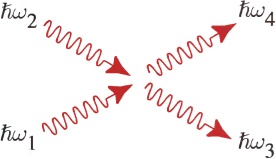
\includegraphics[width=.22\textwidth]{photons.png}
	%\end{wrapfigure}
	\begin{wrapfigure}{r}{0.35\textwidth}
		\vspace{-20pt}
	    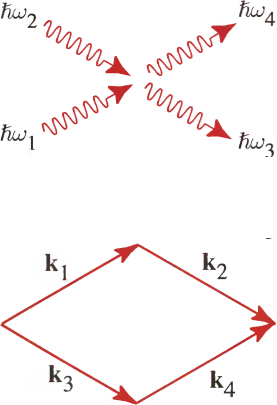
\includegraphics[width=.33\textwidth]{W&K.png}
	\end{wrapfigure}
	FWM uses 3$^{rd}$ order nonlinearity $\chi^{(3)}$.
	%\begin{wrapfigure}{r}{0.22\textwidth}
	%    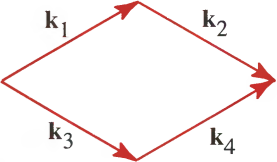
\includegraphics[width=.22\textwidth]{momentum.png}
	%\end{wrapfigure}
	
	\vspace{10pt}
	It consists of the interaction between four EM waves of different frequencies.
	\begin{align}
	\omega_1 + \omega_2 &= \omega_3 + \omega_4\\
	k_1 + k_2 &= k_3 + k_4
	\label{eq_general_f}
	\end{align}
	
	\vspace{5pt}
	Special case:\\ $\omega_1 = \omega_2 = \omega_P$, with stimulation.
\end{frame}
%\subsection{Conservation of energy and momentum}
\begin{frame}{Conservation of energy and momentum}
	\begin{figure}
		\centering
		\vspace{10pt}
		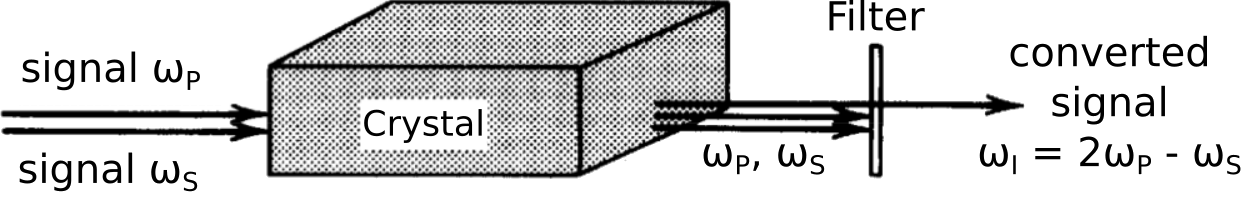
\includegraphics[width=.8\textwidth]{setup_b&w.png}
	\end{figure}
	Conservation of energy is naturally verified
	\begin{equation}
		\omega_I = 2\omega_P - \omega_S = \omega_P \pm \Omega
		\label{eq_energy}
	\end{equation}
	Conservation of momentum is imposed on the phase-mismatch
	\begin{equation}
		\Delta k = 2\,k_P(\omega_P) - k_S(\omega_S) -k_I(\omega_I) = 0
		\label{eq_momentum}
	\end{equation}
	%\begin{equation*}
	%\mathrm{where} \qquad k = \frac{\omega}{c} = \frac{2\pi}{\lambda}
	%\end{equation*}
\end{frame}
\begin{frame}
	Generation happens also for $\Delta k \approx 0$, but at lower efficiency.
	\begin{wrapfigure}{r}{0.5\textwidth}
		\vspace{10pt}
		\centering
	    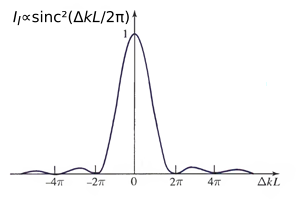
\includegraphics[width=.5\textwidth]{sinc2.png}
	\end{wrapfigure}
	\begin{equation}
	\begin{split}
		I_I &\propto \left| \int_0^L exp(\mathrm{i}\Delta k z)dz\right| \\
			&\propto L^2 sinc(\Delta k / 2\pi)
	\end{split}
	\end{equation}
	We define the coherence length
	\begin{equation}
		L_{coh} = \frac{2\pi}{|\Delta k|}
	\label{eq_coherence_length}
	\end{equation}
\end{frame}
\begin{frame}
	Bulk silicon does not permit to verify both equations.
	\begin{equation}
	k(\omega) = k_0 n(\omega)
	\label{eq_k(w)}
	\end{equation}
	\begin{figure}
		\centering
%		\vspace{-5pt}
		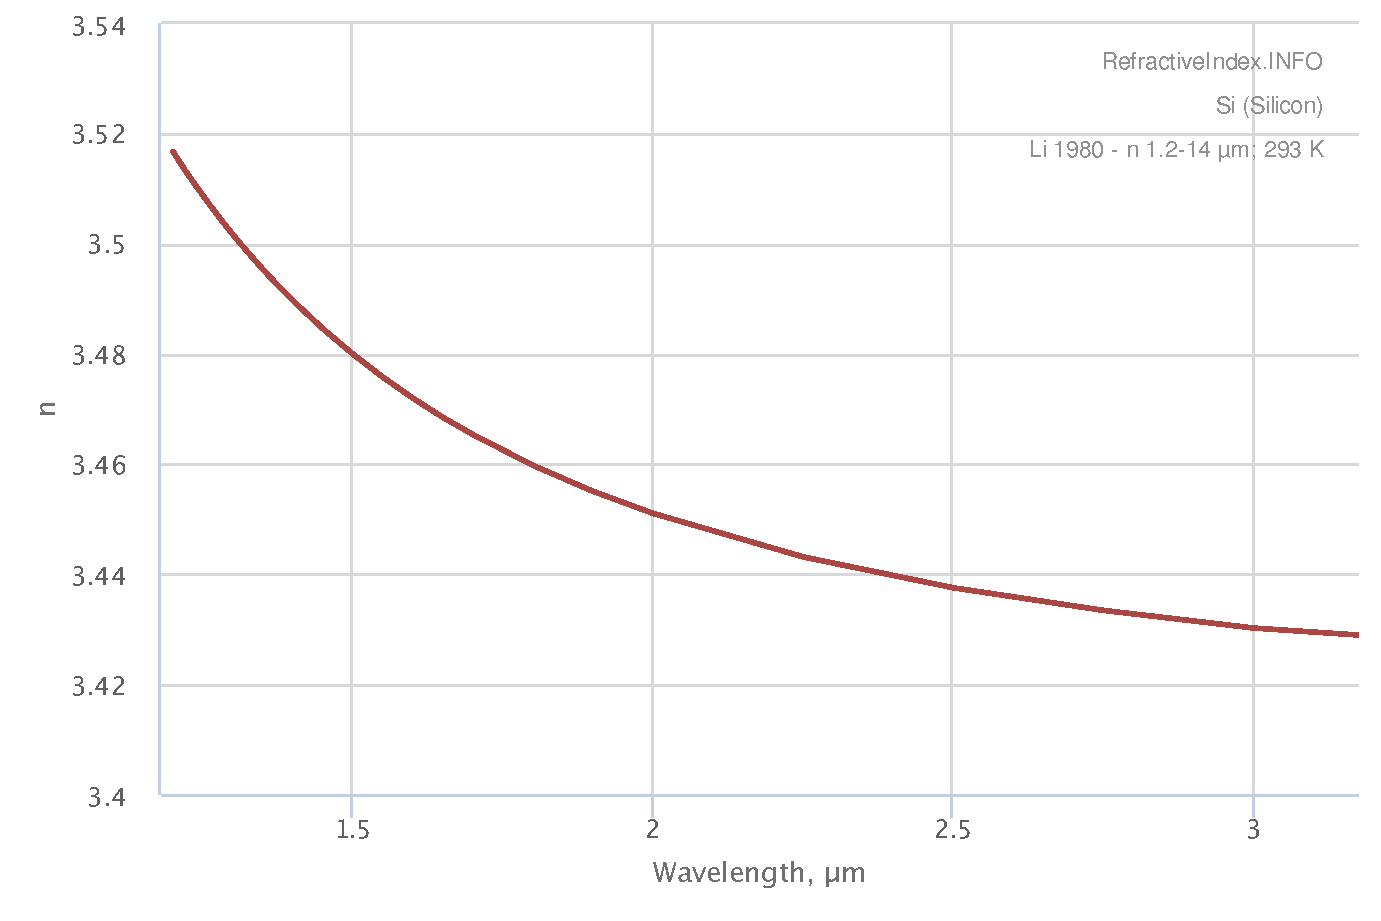
\includegraphics[width=0.8\textwidth]{RefractiveIndexINFO.pdf}
		\label{fig_silicon_dispersion}
	\end{figure}
\end{frame}
%\subsubsection{Multimodal Waveguides}
\begin{frame}{Multimodal Waveguides}
	In silicon waveguides both equations can be verified.\\
	Therefore Eq. \eqref{eq_momentum} becomes:
	\begin{equation}
		\Delta k = 2\,\beta_P(\omega_P) -\beta_S(\omega_S) -\beta_I(\omega_I)
		\label{eq_beta}
	\end{equation}
	\begin{equation*}
		\mathrm{where} \qquad	\beta(\omega) = k_0 n_{eff}(\omega)
	\end{equation*}
	\vspace{-5pt}
	\begin{itemize}
	\item	If the waveguide supports only one mode, phase-matching is only near the frequency of the pump and $\Omega \ll \omega_P$
	\item	If the waveguide is multimodal, there are more matching conditions and also $\Omega \lesssim \omega_P$.
	\end{itemize}
\end{frame}

%\subsection{Phase-matching tuning}
\begin{frame}{Phase-matching tuning}
	\begin{wrapfigure}{r}{0.5\textwidth}
		\vspace{-10pt}
		\centering
	    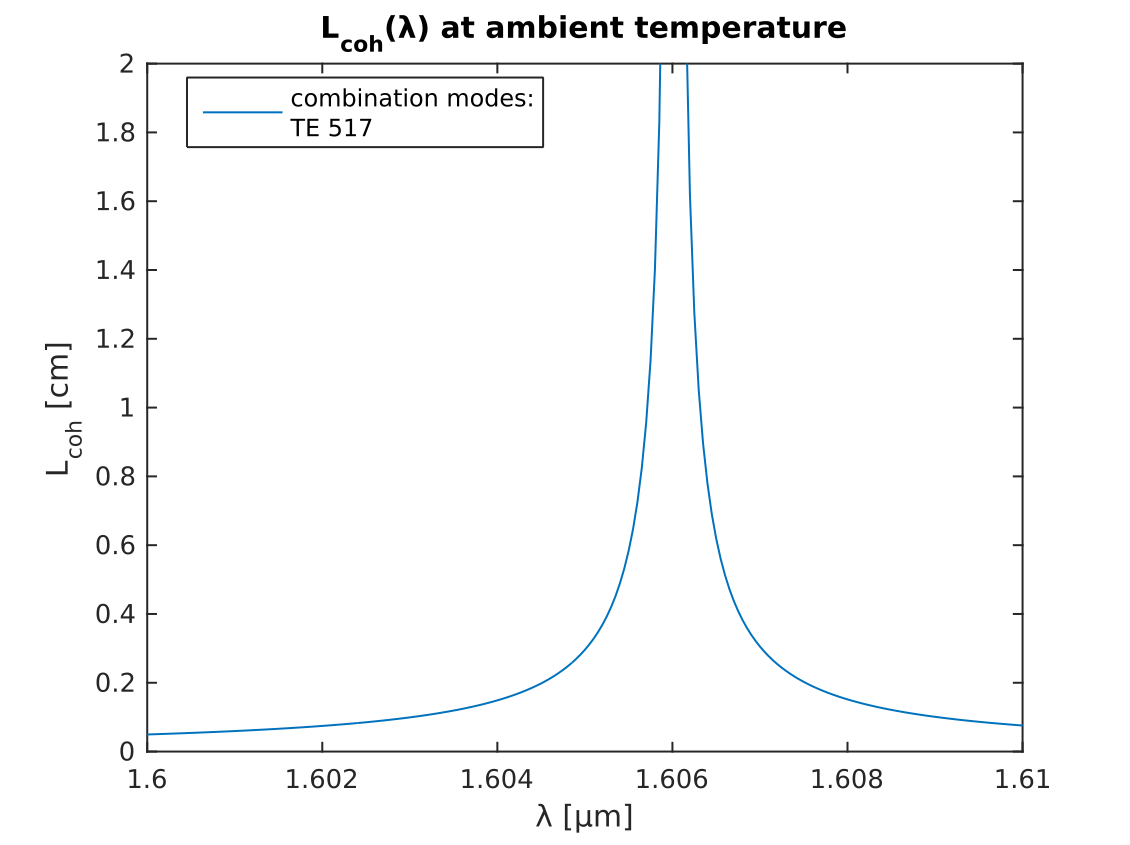
\includegraphics[width=.55\textwidth]{narrow_bandwidth.png}
	\end{wrapfigure}
	Phase-matching conditions have narrow bandwidth.
	
	\vspace{20pt}
	It is difficult to obtain phase-matching at the required wavelength.
	
	\vspace{20pt}
	We aim to tune with temperature the range where phase-matching is verified.
\end{frame}
%\subsubsection{Thermo-Optic Coefficient}
\begin{frame}{Thermo-Optic Coefficient}
	Refractive index of silicon is influenced from the temperature.
	
	\begin{equation}
	\begin{split}
		n 	&= n(\omega,T(x,y)) \\
			&= n(\omega,T_{amb}) + \mathrm{TOC}\cdot(T(x,y)-T_{amb})
		\label{eq_refractive_index}
	\end{split}
	\end{equation}
	
	\vspace{10pt}
	Different modes react differently at the change of temperature.
	\begin{equation}
		n_{eff} = n_{eff}(\omega,T_{amb}) + \mathrm{TOC}_{eff}\cdot(T_H-T_{amb})
		\label{eq_effective_index}
	\end{equation}
\end{frame}
\begin{frame}
	\begin{figure}
		\centering
		\vspace{-10pt}
		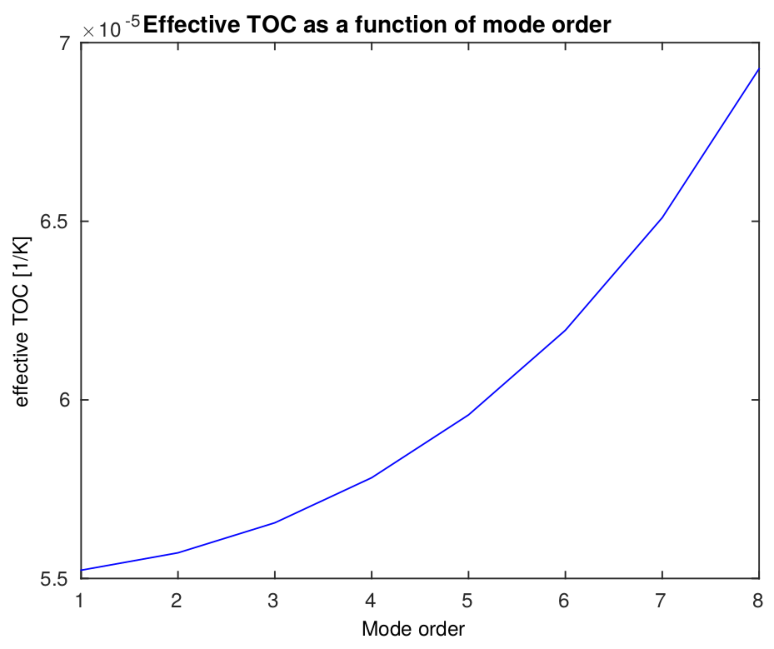
\includegraphics[width=.8\textwidth]{effectiveTOC.pdf}
		\label{fig_TOC_effective}
		\vspace{-10pt}
	\end{figure}
	It should be possible to control phase-matching with temperature.
\end{frame}
\section{Computational model}
\begin{frame}{Computational model}
	\begin{figure}
%		\vspace{-15pt}
		\centering
		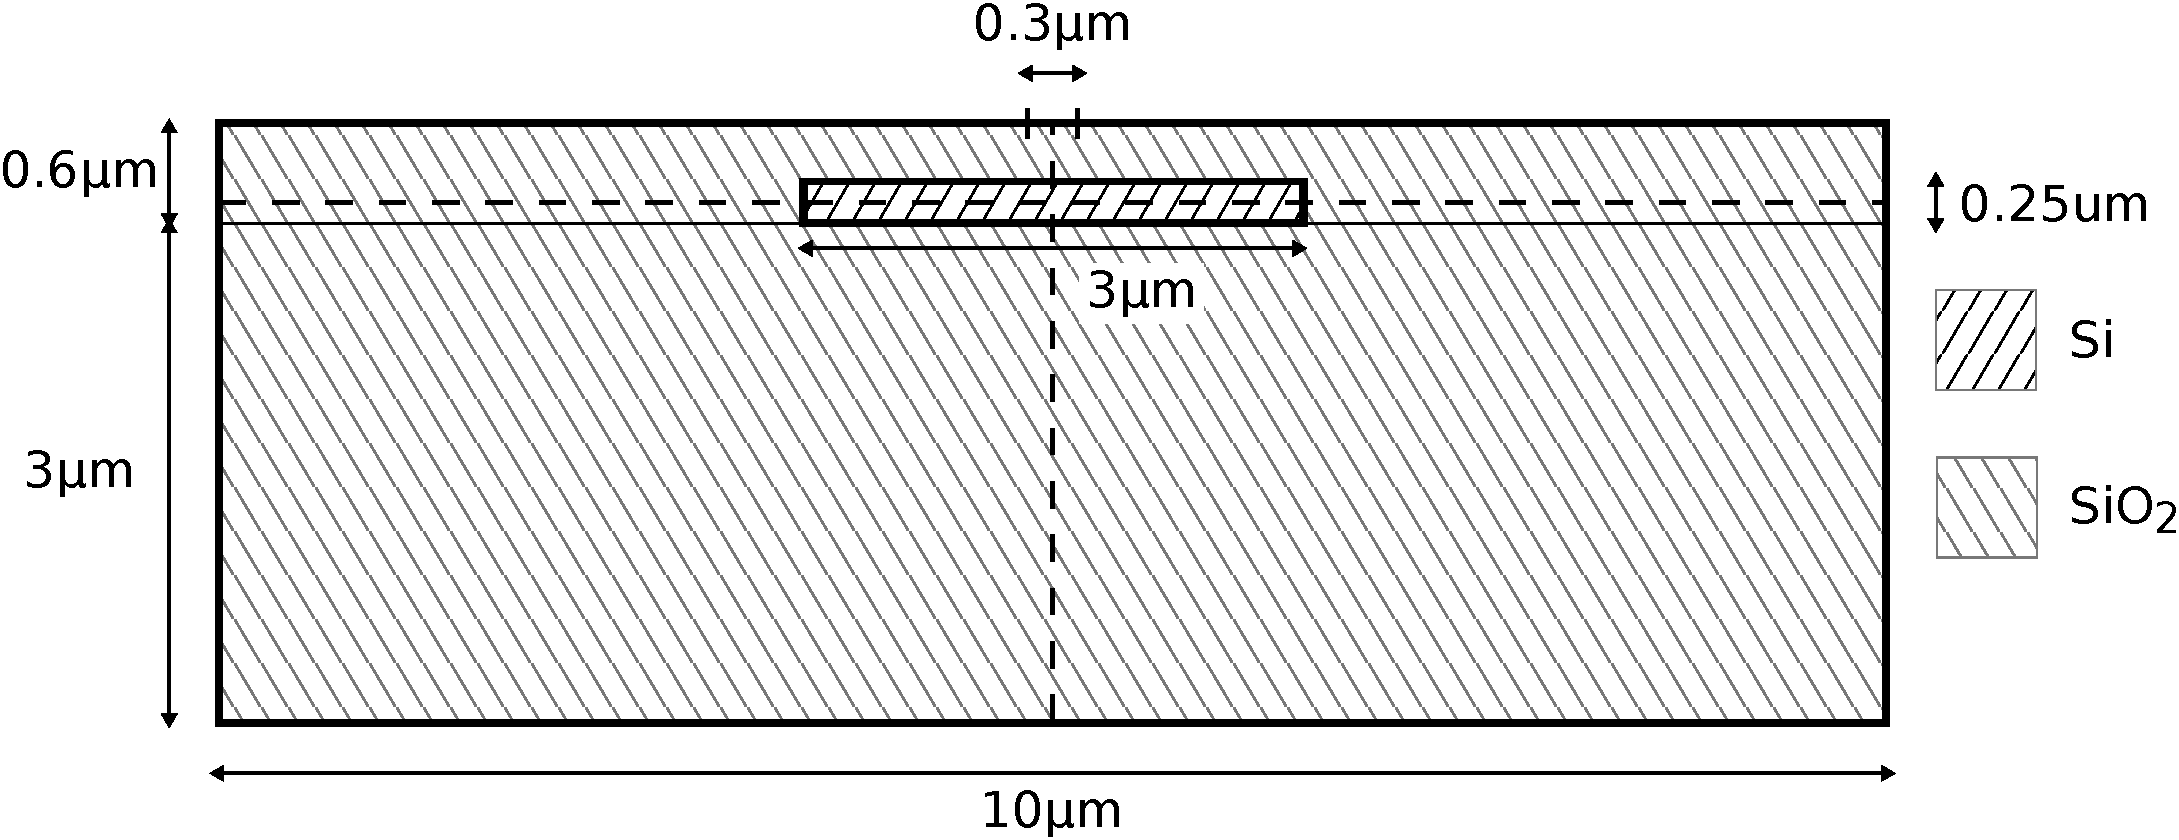
\includegraphics[width=\textwidth]{geometry.pdf}
	\end{figure}
\end{frame}
%\subsection{Temperature simulation}
\begin{frame}{Temperature simulation}
	\begin{figure}
%		\vspace{-15pt}
		\centering
		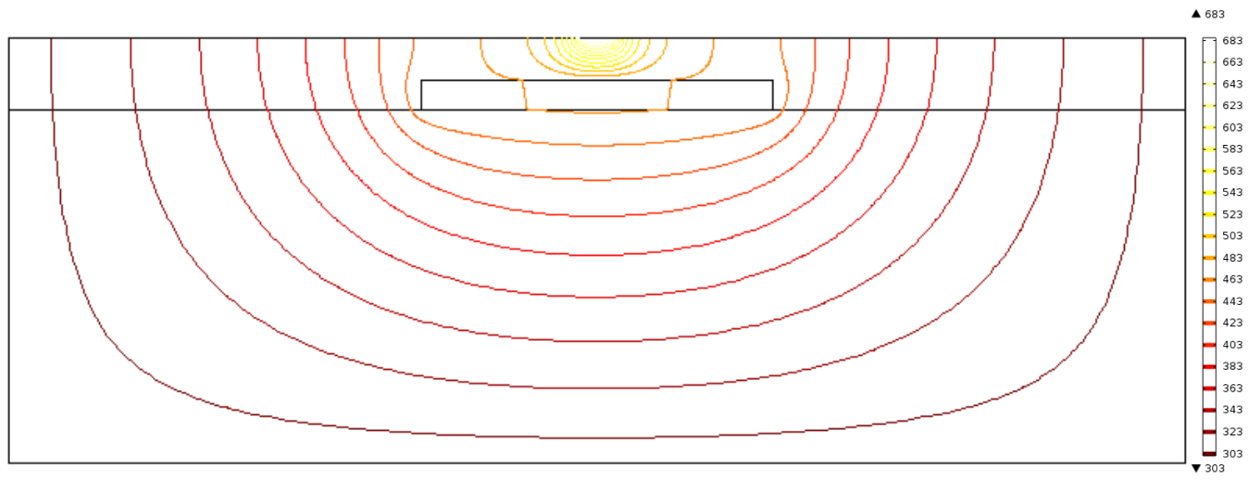
\includegraphics[width=\textwidth]{thermal.pdf}
	\end{figure}
\end{frame}
%\subsection{Mode simulation}
\begin{frame}{Mode simulation}
	\begin{figure}
%		\vspace{-15pt}
		\centering
		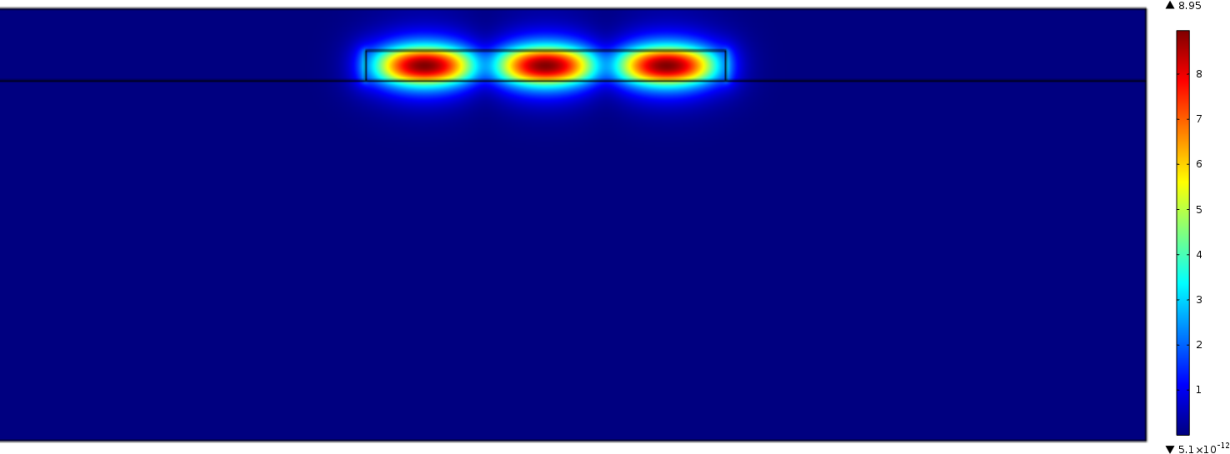
\includegraphics[width=\textwidth]{output_modeTE.pdf}
	\end{figure}
\end{frame}
\begin{frame}{Mode simulation}
	\begin{figure}
%		\vspace{-15pt}
		\centering
		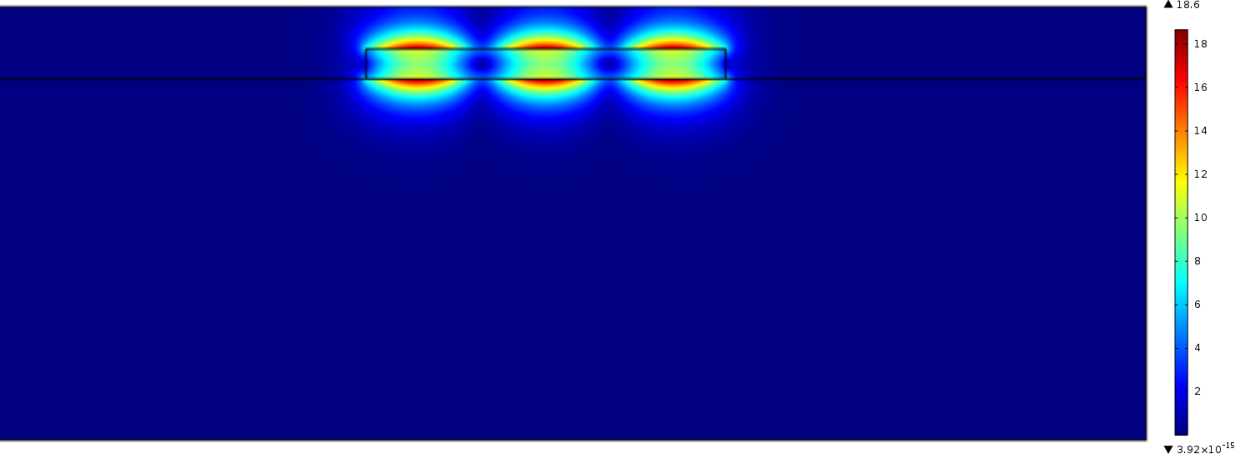
\includegraphics[width=\textwidth]{output_modeTM.pdf}
	\end{figure}
\end{frame}
\section{Data analysis}
\begin{frame}{Data analysis}
	\begin{itemize}
	\item	Data extraction from comsol to matlab.
	\item	Data classification (TE/TM, order).
	\item	Data processing:\\
			\begin{itemize}
			\item	polynomial fit of $\lambda$ and $T_H$.
			\item	evaluation of phase-mismatch \eqref{eq_momentum} with \eqref{eq_beta} and \eqref{eq_effective_index}
					\begin{equation}
					\Delta k = 2	 \frac{2\pi}{ \lambda_P } n_{eff}(\lambda_P,T_H)
								-\frac{2\pi}{ \lambda_S } n_{eff}(\lambda_S,T_H)
								-\frac{2\pi}{ \lambda_I } n_{eff}(\lambda_I,T_H)
					\end{equation}
					and coherence length $L_{coh} = \frac{2\pi}{|\Delta k|}$.
			\end{itemize}
	\item	Data selection: verify condition $L_{coh}/L_{sam} \geq 1$.
	\item	Data aggregation.
	\end{itemize}
\end{frame}
\section{Results}
\begin{frame}{Results: symmetric configuration}
	\begin{figure}
%		\vspace{-15pt}
		\centering
		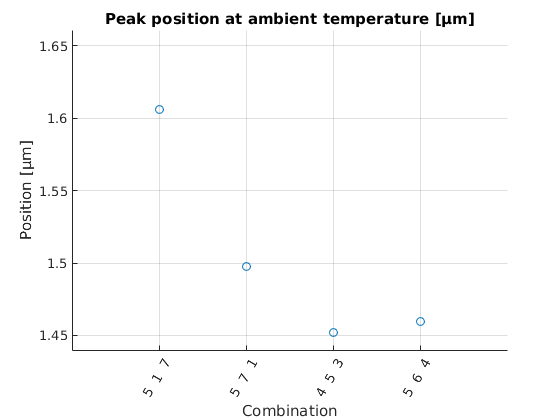
\includegraphics[height=.8\textheight]{ppaat22.png}
	\end{figure}
\end{frame}
\begin{frame}
	\begin{figure}
%		\vspace{-15pt}
		\centering
		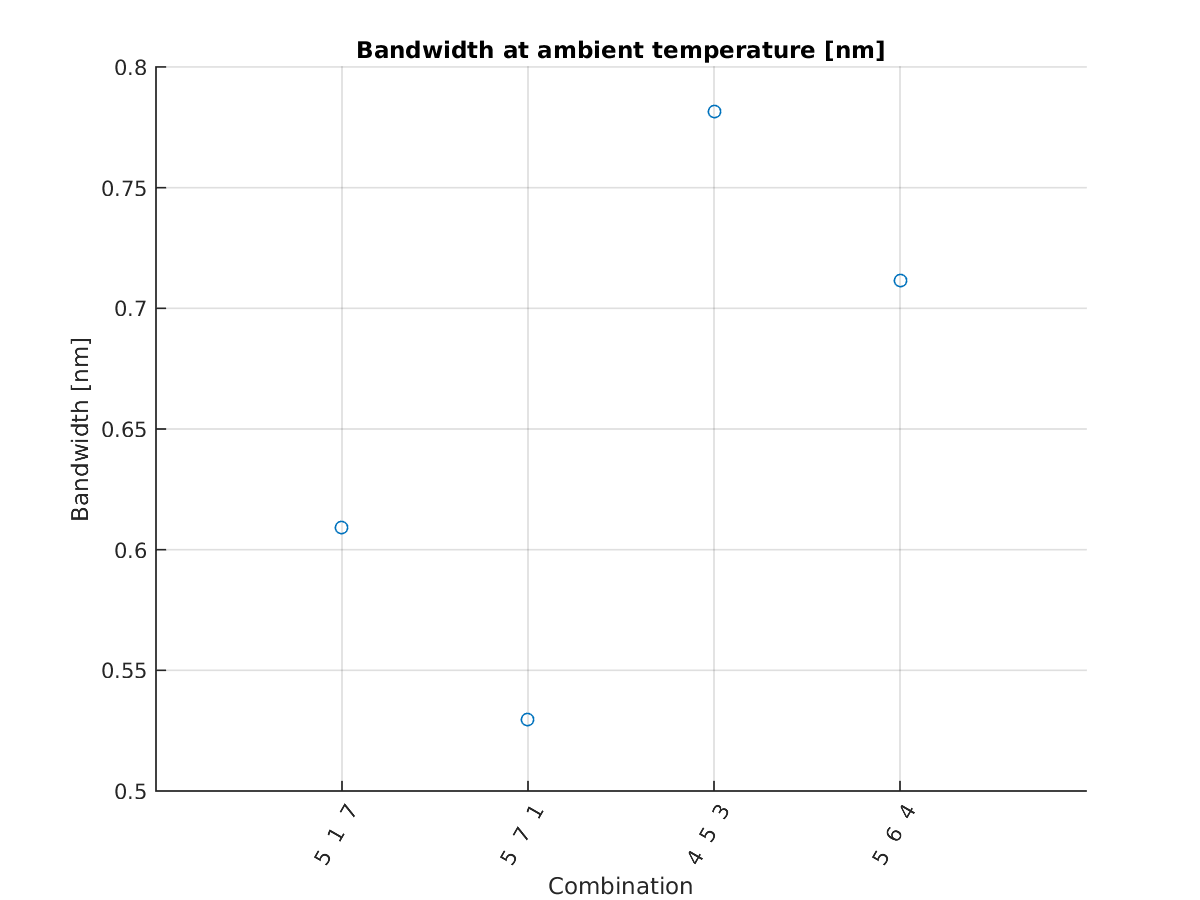
\includegraphics[height=.9\textheight]{baat2.png}
	\end{figure}
\end{frame}
\begin{frame}
	\begin{figure}
%		\vspace{-15pt}
		\centering
		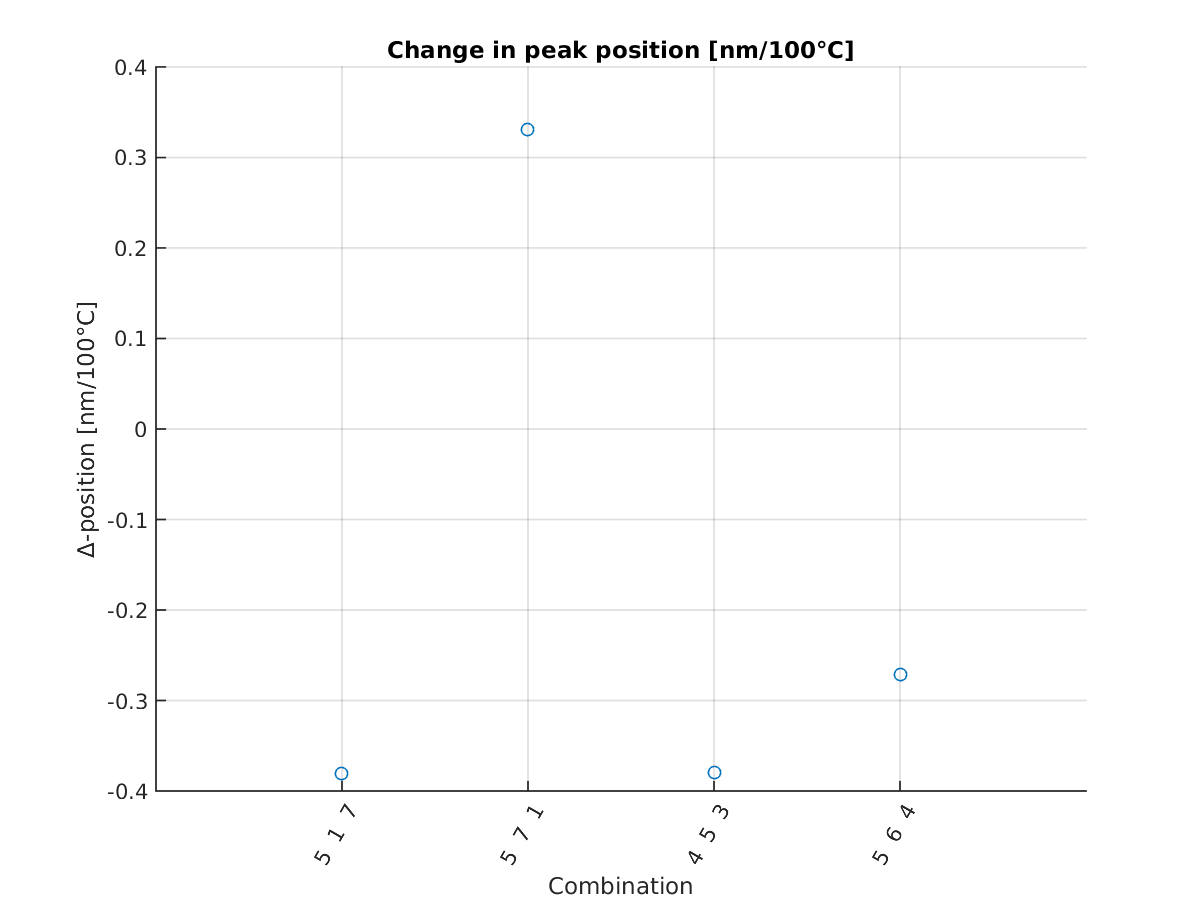
\includegraphics[height=.9\textheight]{ppc2.png}
	\end{figure}
\end{frame}
\begin{frame}
	Combination \texttt{TE 517}, symmetric configuration.
	\begin{figure}
%		\vspace{-15pt}
		\centering
		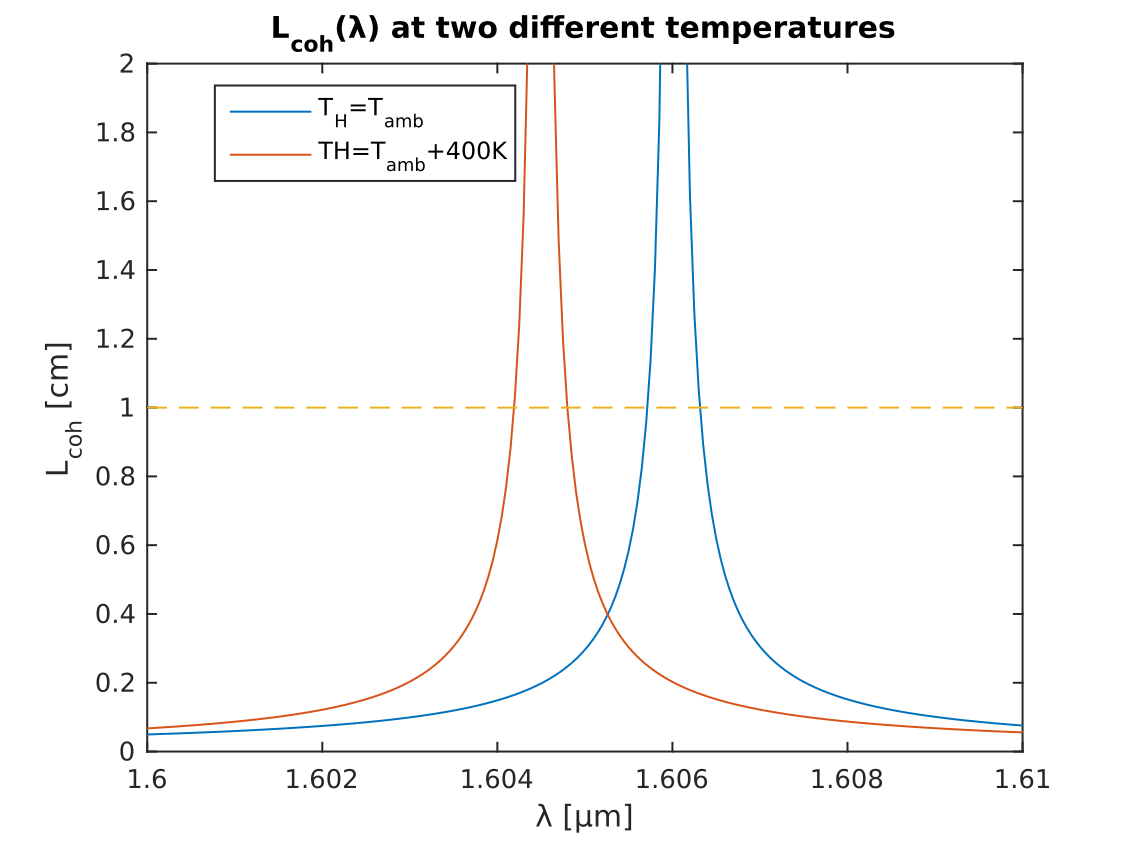
\includegraphics[width=.8\textwidth]{bandwidth_movement_TE517_sym.png}
	\end{figure}
\end{frame}
\begin{frame}{Asymmetric configuration}
	\begin{figure}
%		\vspace{-15pt}
		\centering
		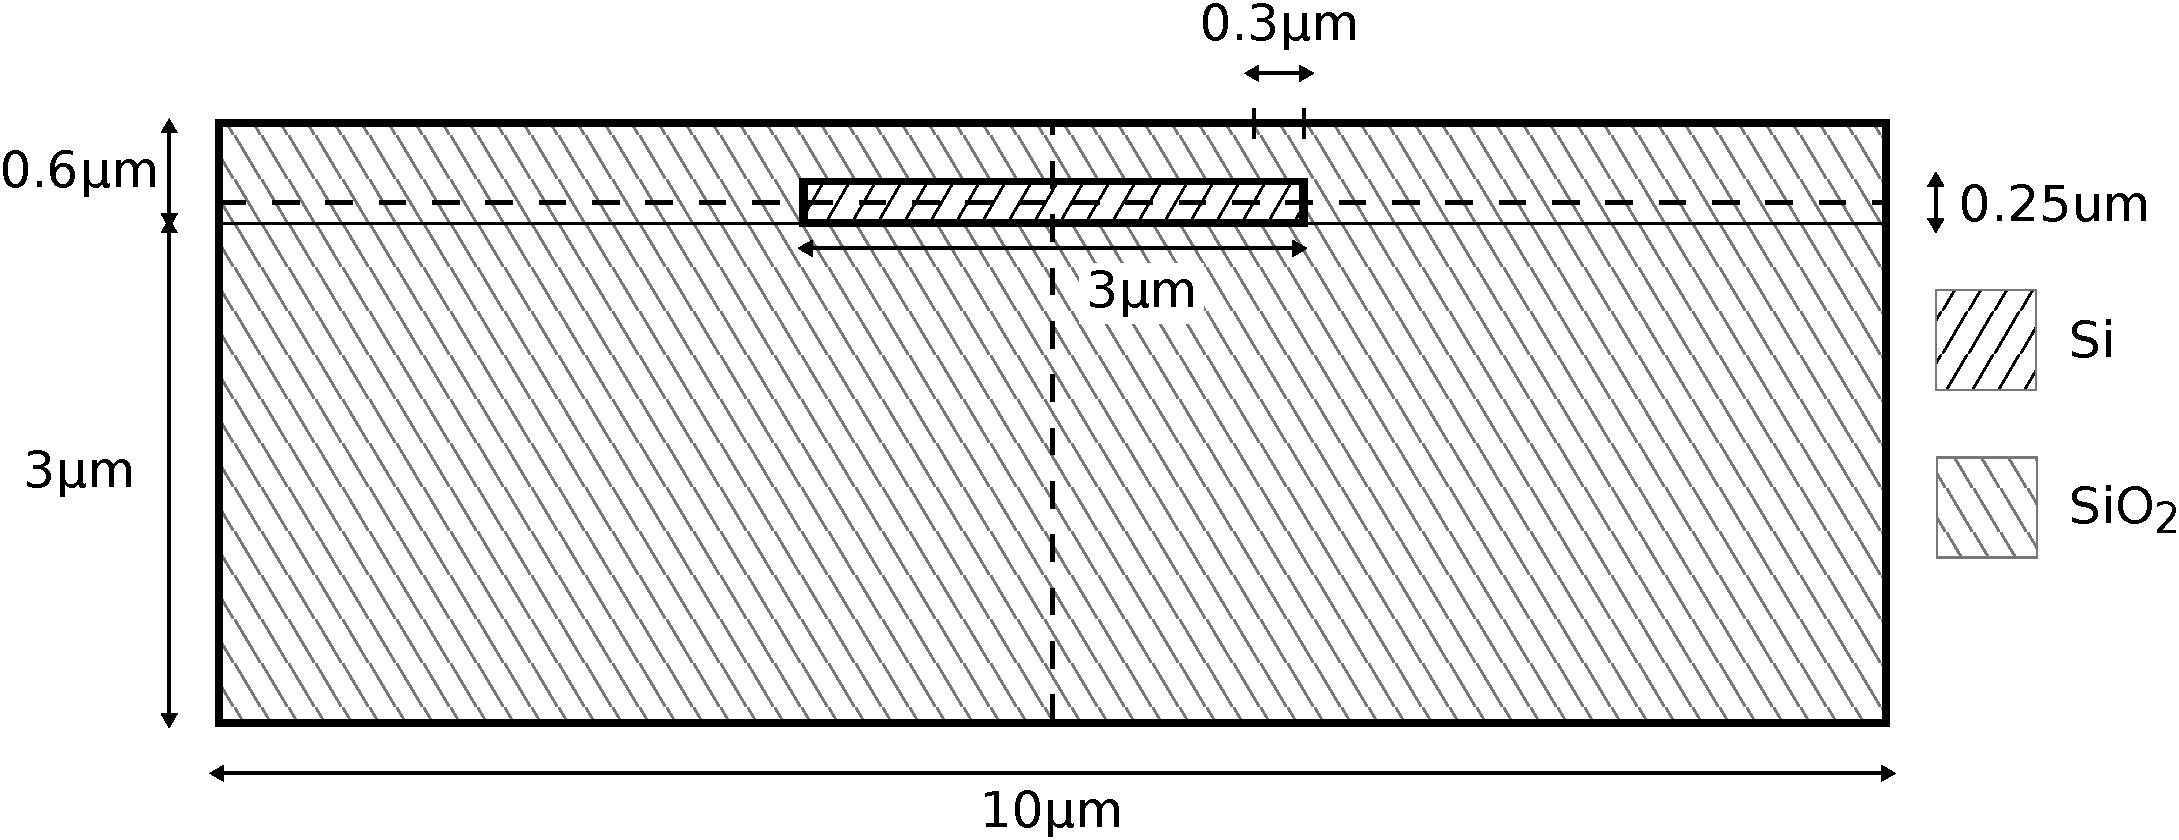
\includegraphics[width=\textwidth]{geometryA.pdf}
	\end{figure}
\end{frame}
\begin{frame}
	\begin{figure}
%		\vspace{-15pt}
		\centering
		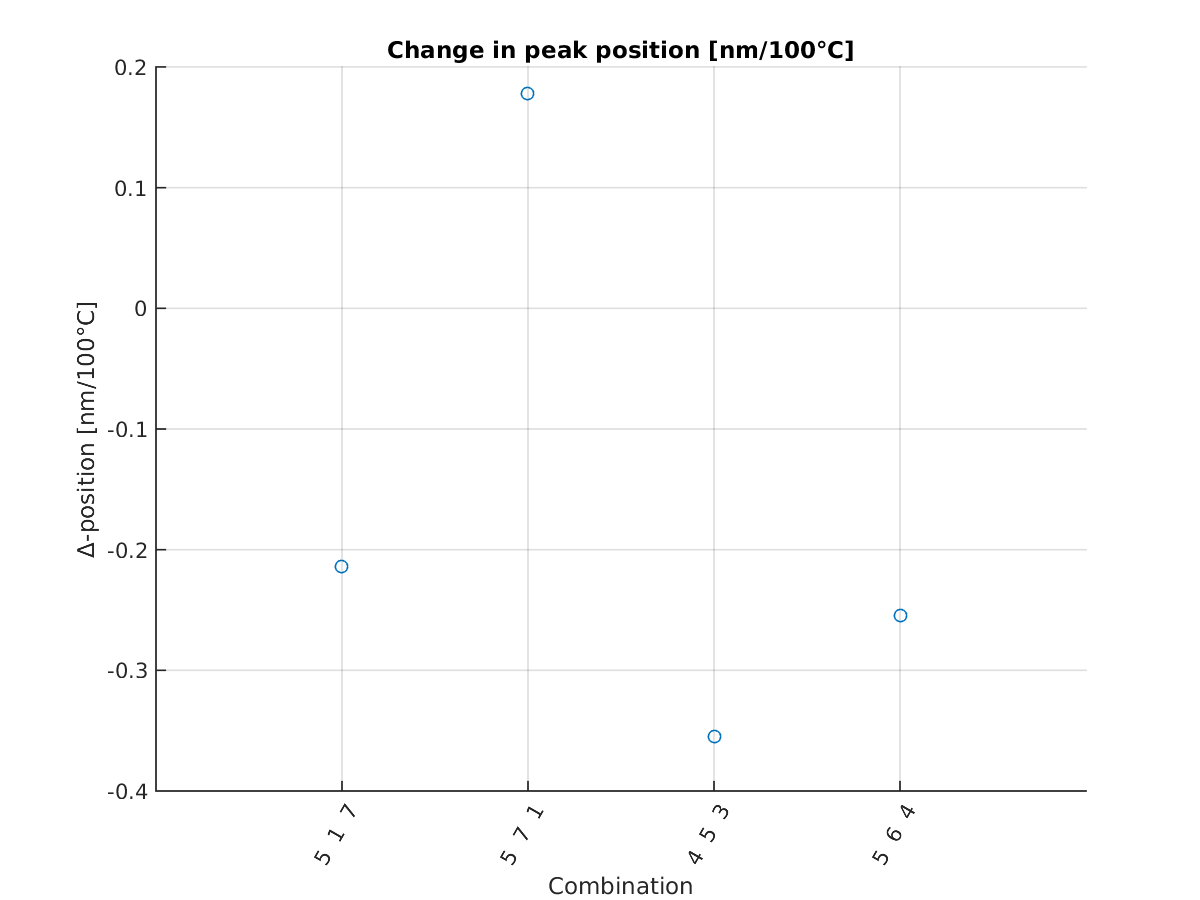
\includegraphics[height=.85\textheight]{asym_ppc2.png}
	\end{figure}
\end{frame}
\section{Conclusion}
%\subsection{Improvements}
\begin{frame}{Improvements}
	\begin{itemize}
		\item	The heater should be simulated as a metal conductor media, instead of a simple boundary condition (TM modes).
		\item	Thermo-Optic Coefficient also depends on the wavelength of the signal.
		\item	Different core geometries should be studied.
		\item	Develop the correlation also between temperature and efficiency of energy conversion.
	\end{itemize}
\end{frame}
%\subsection{Summary}
\begin{frame}{Summary}
	\begin{itemize}
		\item Configurations with a high difference between their orders are to be preferred.
		\item Limited interaction between the temperature of material and different modes is a constraint.
		\item Thermal tuning of the FWM phase-match is, in fact, possible.
	\end{itemize}
\end{frame}
\end{document}